\chapter{Blockchain}
The basic concepts concerning Blockchains are
\begin{itemize}
   \item \textit{Ledger}
   \item \textit{Consensus} in a distributed environment
   \item Tamper freeness
   \item Proof of ownership
   \item Permissioned and permissionless blockchains
\end{itemize}

Each \textbf{block} is made up of \textit{Data}, \textit{Hash} and the \textit{Hash of the previous block}; pointers to the previous block are used to ensure the \textbf{order} of the blocks, resulting in a \textbf{chain} of blocks.

\textbf{Tamper freeness} refers to changing one hash causes changing the hash of the following blocks, implying not only to recompute some hashes, but also to find a value that combined with the new hash solves the \textit{Proof of Work}.

\begin{figure}[htbp]
   \centering
   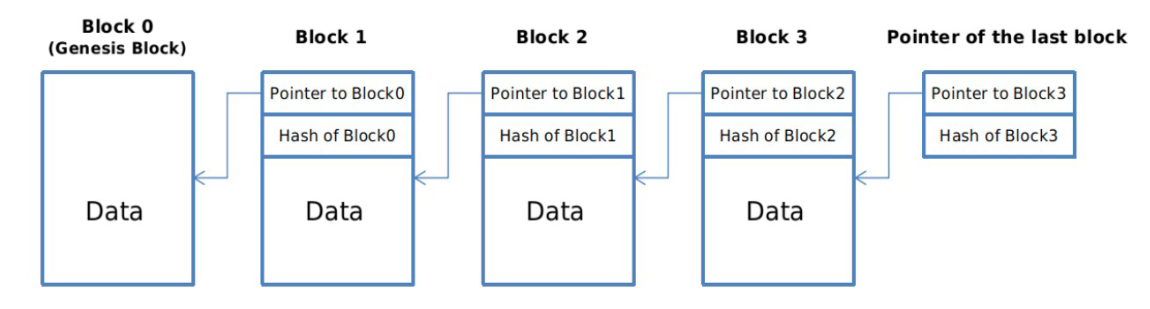
\includegraphics{images/hashpointers.png}
   \caption{Hash pointers and hash of the block prevent attackers from tampering with the blockchain}
   \label{fig:hashpointers}
\end{figure}

A \textbf{ledger}\footnote{\textit{``Libro mastro''} in italiano} acts like a notary, and is replicated on each node of a P2P network, it is immutable and benefits of the tamper freeness property.\\
The ledger is like a bullettin storing operations and their order. It must be an \textbf{append-only} list of events, and also \textbf{tamper-proof}.

\begin{center}
   \ul{If a ledger is organized as a list of blocks, we call it a \textbf{blockchain}}.
\end{center}
\nl

\section{Consesus and challenges}
\textbf{Consensus} is the mechanism which defines who decides which operation will be added to the blockchain, and which operation among those to be confirmed will be added.
Consesus is implemented by \textit{voting}, but there a few things to handle to avoid double spending and fake votes.
\textit{Sybil} attacks are a common issue in voting systems, where a single node can fake multiple identities to gain more voting power.

The two main challenges for the ledger are keeping consistency in case of network jitter and possible delays, and avoid nodes to fake results.
An idea is to establish \textit{consensus} using a \textbf{Proof of Work}, which requires the voting system to be hardly fakeable, i.e. resolving a difficult computational problem.
Enforcing a \textit{PoW} is a way to avoid the Sybil attacks issue, as it implies to have a lot of computational power to fake a vote.\\
The Proof of Work is often compared to a lottery, where tickets for the lottery are very expensive (computational power), and the winner is the one who solves the problem first, and gets the right to decide which block to add to the blockchain.

In case multiple winners are picked at the same time, a \textbf{fork} is created, and the network must decide which fork to follow. The longest fork is usually the one to be followed, as it is the one with the most computational power behind it.

\section{Restricted access}
It is possible to build a permissioned blockchain, where only a restricted set of nodes can vote and add blocks to the blockchain. This is useful in case of a consortium of companies, where the blockchain is used to store transactions between them.

The blockchain may be exploited to demonstrate the validity of the supply chain of a product, or to store the history of a product, from the raw materials to the final product, allowing also to determine which point in the supply chain a product has been compromised.